\documentclass{beamer}\usepackage[]{graphicx}\usepackage[]{color}
%% maxwidth is the original width if it is less than linewidth
%% otherwise use linewidth (to make sure the graphics do not exceed the margin)
\makeatletter
\def\maxwidth{ %
  \ifdim\Gin@nat@width>\linewidth
    \linewidth
  \else
    \Gin@nat@width
  \fi
}
\makeatother

\definecolor{fgcolor}{rgb}{0.345, 0.345, 0.345}
\newcommand{\hlnum}[1]{\textcolor[rgb]{0.686,0.059,0.569}{#1}}%
\newcommand{\hlstr}[1]{\textcolor[rgb]{0.192,0.494,0.8}{#1}}%
\newcommand{\hlcom}[1]{\textcolor[rgb]{0.678,0.584,0.686}{\textit{#1}}}%
\newcommand{\hlopt}[1]{\textcolor[rgb]{0,0,0}{#1}}%
\newcommand{\hlstd}[1]{\textcolor[rgb]{0.345,0.345,0.345}{#1}}%
\newcommand{\hlkwa}[1]{\textcolor[rgb]{0.161,0.373,0.58}{\textbf{#1}}}%
\newcommand{\hlkwb}[1]{\textcolor[rgb]{0.69,0.353,0.396}{#1}}%
\newcommand{\hlkwc}[1]{\textcolor[rgb]{0.333,0.667,0.333}{#1}}%
\newcommand{\hlkwd}[1]{\textcolor[rgb]{0.737,0.353,0.396}{\textbf{#1}}}%

\usepackage{framed}
\makeatletter
\newenvironment{kframe}{%
 \def\at@end@of@kframe{}%
 \ifinner\ifhmode%
  \def\at@end@of@kframe{\end{minipage}}%
  \begin{minipage}{\columnwidth}%
 \fi\fi%
 \def\FrameCommand##1{\hskip\@totalleftmargin \hskip-\fboxsep
 \colorbox{shadecolor}{##1}\hskip-\fboxsep
     % There is no \\@totalrightmargin, so:
     \hskip-\linewidth \hskip-\@totalleftmargin \hskip\columnwidth}%
 \MakeFramed {\advance\hsize-\width
   \@totalleftmargin\z@ \linewidth\hsize
   \@setminipage}}%
 {\par\unskip\endMakeFramed%
 \at@end@of@kframe}
\makeatother

\definecolor{shadecolor}{rgb}{.97, .97, .97}
\definecolor{messagecolor}{rgb}{0, 0, 0}
\definecolor{warningcolor}{rgb}{1, 0, 1}
\definecolor{errorcolor}{rgb}{1, 0, 0}
\newenvironment{knitrout}{}{} % an empty environment to be redefined in TeX

\usepackage{alltt}
\usetheme[compress]{Singapore}
\useoutertheme{miniframes}

% \documentclass{beamer}
%\usetheme{Warsaw}

% Pour les documents en francais...
	\usepackage[latin1]{inputenc}
	\usepackage[french]{babel}
	\usepackage[french]{varioref}

% Math�matiques
	\usepackage{amsmath}

% Caracteres speciaux suppl�mentaires
	\usepackage{latexsym,amsfonts}

% A documenter
	\usepackage{moreverb}

% Macros pour les paquets
	\usepackage{array}  			% N�cessaires pour les tableaux de la macro Excel.

% Outil suppl�mentaire pour les tableaux
	\usepackage{multirow}
	\usepackage{booktabs}
	\usepackage{xcolor} % alternating row colors in table, incompatible avec certains modules
	\usepackage{longtable}
	\usepackage{colortbl}

% Pour ins�rer des graphiques
	\usepackage{graphicx} 			% Graphique simples
	\usepackage{subfigure}			% Graphiques multiples

% Pour ins�rer des couleurs
	\usepackage{color}

% Rotation des objets et des pages
%	\usepackage{rotating}
%	\usepackage{lscape}

% Pour insrer du code source, LaTeX ou SAS par exemple.
	\usepackage{verbatim}
        \usepackage{moreverb}
	\usepackage{listings}
	\usepackage{fancyvrb}

%	\lstset{language=SAS,numbers=left}		% Par dfaut le listing est en SAS

% Pour ins�rer des hyperliens
  \usepackage{hyperref}

% American Psychological Association (for bibliographic references).
	\usepackage{apacite}

% Pour l'utilisation des macros
	\usepackage{xspace}

% Pour l'utilisation de notes en fin de document.
%	\usepackage{endnotes}

% Array
%	\usepackage{multirow}
%	\usepackage{booktabs}

% Rotation
%	\usepackage{rotating}

% En t�tes et pieds de pages
%	\usepackage{fancyhdr}
%	\usepackage{lastpage}


% Page layout

% By LaTeX commands
%\setlength{\oddsidemargin}{0cm}
%\setlength{\textwidth}{16cm}
%\setlength{\textheight}{24cm}
%\setlength{\topmargin}{-1cm}
%\setlength{\marginparsep}{0.2cm}

% fancyheader parameters
%\pagestyle{fancy}

%\fancyfoot[L]{{\small Formation \LaTeX, DEPP}}
%\fancyfoot[c]{}
%\fancyfoot[R]{{\small \thepage/\pageref{LastPage}}}

%\fancyhead[L]{}
%\fancyhead[c]{}
%\fancyhead[R]{}


% Pour ins�rer des dessins de Linux
\newcommand{\LinuxA}{\includegraphics[height=0.5cm]{Graphiques/linux.png}}
\newcommand{\LinuxB}{\includegraphics[height=0.5cm]{Graphiques/linux.png}\xspace}

% Macro pour les petits dessins pour les diff�rents OS.
\newcommand{\Windows}{\emph{Windows}\xspace}
\newcommand{\Mac}{\emph{Mac OS X}\xspace}
\newcommand{\Linux}{\emph{Linux}\xspace}
\newcommand{\MikTeX}{MiK\tex\xspace}

\newcommand{\df}{\emph{data.frame}\xspace}
\newcommand{\dfs}{\emph{data.frames}\xspace}
\newcommand{\liste}{\emph{list}\xspace}
\newcommand{\listes}{\emph{lists}\xspace}

\newcommand{\factor}{\emph{factor}\xspace}
\newcommand{\character}{\emph{character}\xspace}
\newcommand{\logical}{\emph{logical}\xspace}

\newcommand{\cad}{c'est-�-dire\xspace}

\newcommand{\hreff}[2]{\underline{\href{#1}{#2}\xspace}}


% Titre
\title{Introduction � R}
\author{Pascal Bessonneau}
%\institute{DEPP}
\date{06/2015}
\subtitle{ACP}

\begin{knitrout}
\definecolor{shadecolor}{rgb}{0.969, 0.969, 0.969}\color{fgcolor}\begin{kframe}


{\ttfamily\noindent\itshape\color{messagecolor}{\#\# Loading required package: FactoMineR}}\end{kframe}
\end{knitrout}

\IfFileExists{upquote.sty}{\usepackage{upquote}}{}
\begin{document}

\begin{frame}
	\maketitle
\end{frame}

\begin{frame}
	\tableofcontents
\end{frame}

% Begin document %%%%%%%%%%%%%%%%%%%%%%%%%%%%%%%%%%%%%%%%%%%%%%%%%%%%%%%%%%%%%%%%%%%%%%%%%%%%%%%%%%

\section{Analyse en composante principale}

\begin{frame}[containsverbatim]
	\frametitle{Le principe}

  Les d�tails math�matiques ne seront pas pr�sent�s. Il s'agit juste de montrer
  comment on peut synth�tiser un probl�me avec des variables artificielles
  dont le nombre est inf�rieur ou tr�s inf�rieure au nombre de variables
  initiales qui d�crivent les individus.
  
\end{frame}

\begin{frame}[containsverbatim]
	\frametitle{Temp�rature}

\begin{knitrout}\footnotesize
\definecolor{shadecolor}{rgb}{0.969, 0.969, 0.969}\color{fgcolor}\begin{kframe}
\begin{alltt}
\hlstd{temp} \hlkwb{<-} \hlkwd{read.csv2}\hlstd{(}\hlstr{"data/temp.csv"}\hlstd{)}
\hlkwd{colnames}\hlstd{(temp)}
\end{alltt}
\begin{verbatim}
##  [1] "Ville"     "Janvier"   "Fevrier"  
##  [4] "Mars"      "Avril"     "Mai"      
##  [7] "Juin"      "Juillet"   "Aout"     
## [10] "Septembre" "Octobre"   "Novembre" 
## [13] "Decembre"  "lati"      "long"
\end{verbatim}
\end{kframe}
\end{knitrout}

\end{frame}

\begin{frame}[containsverbatim]
	\frametitle{Temp�rature}

\begin{knitrout}\footnotesize
\definecolor{shadecolor}{rgb}{0.969, 0.969, 0.969}\color{fgcolor}\begin{kframe}
\begin{alltt}
\hlkwd{head}\hlstd{(temp)}
\end{alltt}
\begin{verbatim}
##              Ville Janvier Fevrier Mars Avril
## 1         Bordeaux     5.6     6.6 10.3  12.8
## 2            Brest     6.1     5.8  7.8   9.2
## 3 Clermont-Ferrand     2.6     3.7  7.5  10.3
## 4         Grenoble     1.5     3.2  7.7  10.6
## 5            Lille     2.4     2.9  6.0   8.9
## 6             Lyon     2.1     3.3  7.7  10.9
##    Mai Juin Juillet Aout Septembre Octobre
## 1 15.8 19.3    20.9 21.0      18.6    13.8
## 2 11.6 14.4    15.6 16.0      14.7    12.0
## 3 13.8 17.3    19.4 19.1      16.2    11.2
## 4 14.5 17.8    20.1 19.5      16.7    11.4
## 5 12.4 15.3    17.1 17.1      14.7    10.4
## 6 14.9 18.5    20.7 20.1      16.9    11.4
##   Novembre Decembre  lati  long
## 1      9.1      6.2 44.50 -0.34
## 2      9.0      7.0 48.24 -4.29
## 3      6.6      3.6 45.47  3.05
## 4      6.5      2.3 45.10  5.43
## 5      6.1      3.5 50.38  3.04
## 6      6.7      3.1 45.45  4.51
\end{verbatim}
\end{kframe}
\end{knitrout}

\end{frame}

\begin{frame}[containsverbatim]
	\frametitle{Les donn�es}
	
	Ce sont donc les donn�es qui correspondent aux temp�ratures moyennes
	tout au long de l'ann�e pour des villes de France.

\end{frame}

\begin{frame}[containsverbatim]
  \frametitle{Peut-on r�sumer les informations ?}

Le principe de l'ACP est de chercher et de simplifier les corr�lations qui existe
entre les variables pour cr�er des variables synth�tiques qui avec peu 
de nouvelles variables r�sumeront le maximum d'informations possibles.

Pour r�aliser l'analyse on utilise le paquet FactoMineR.

\end{frame}

\begin{frame}[containsverbatim]
	\frametitle{Pr�paration des donn�es}

\begin{knitrout}\footnotesize
\definecolor{shadecolor}{rgb}{0.969, 0.969, 0.969}\color{fgcolor}\begin{kframe}
\begin{alltt}
\hlkwd{rownames}\hlstd{(temp)} \hlkwb{<-} \hlstd{temp}\hlopt{$}\hlstd{Ville}
\hlstd{temp} \hlkwb{<-} \hlstd{temp[,}\hlopt{-}\hlnum{1}\hlstd{]}
\end{alltt}
\end{kframe}
\end{knitrout}

\end{frame}

\begin{frame}[containsverbatim]
  \frametitle{Graphiques des variables}

\begin{knitrout}\footnotesize
\definecolor{shadecolor}{rgb}{0.969, 0.969, 0.969}\color{fgcolor}\begin{kframe}
\begin{alltt}
\hlstd{pca} \hlkwb{<-} \hlkwd{PCA}\hlstd{(temp,}\hlkwc{quanti.sup} \hlstd{=} \hlkwd{c}\hlstd{(}\hlnum{13}\hlstd{,}\hlnum{14}\hlstd{))}
\end{alltt}
\end{kframe}

{\centering 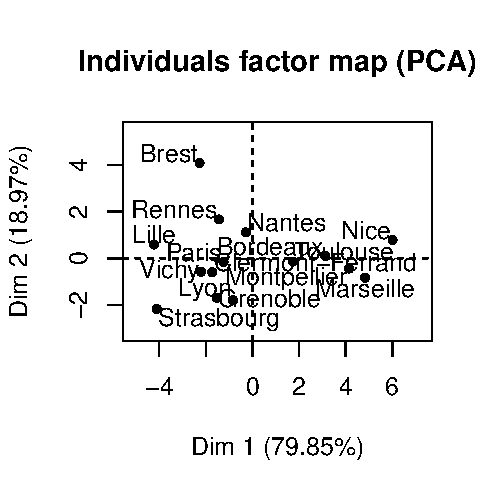
\includegraphics[width=\textwidth]{graphiques/beamer-unnamed-chunk-5-1} 
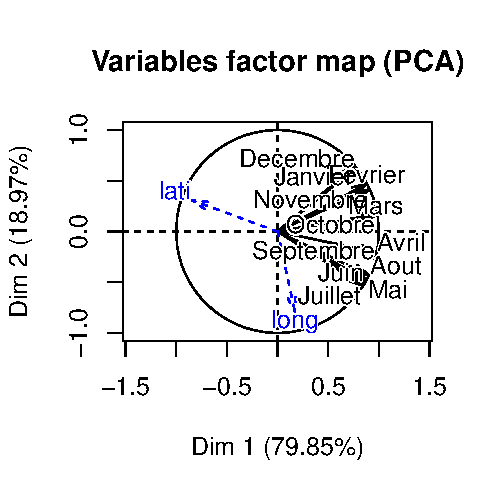
\includegraphics[width=\textwidth]{graphiques/beamer-unnamed-chunk-5-2} 

}



\end{knitrout}

colnames(temp)  
  
\end{frame}

\begin{frame}[containsverbatim]
  \frametitle{Graphique des  individus sur les deux premiers axes}

\begin{knitrout}\footnotesize
\definecolor{shadecolor}{rgb}{0.969, 0.969, 0.969}\color{fgcolor}\begin{kframe}
\begin{alltt}
\hlkwd{plot}\hlstd{(pca,}\hlkwc{choix} \hlstd{=} \hlstr{"ind"}\hlstd{)}
\end{alltt}
\end{kframe}

{\centering 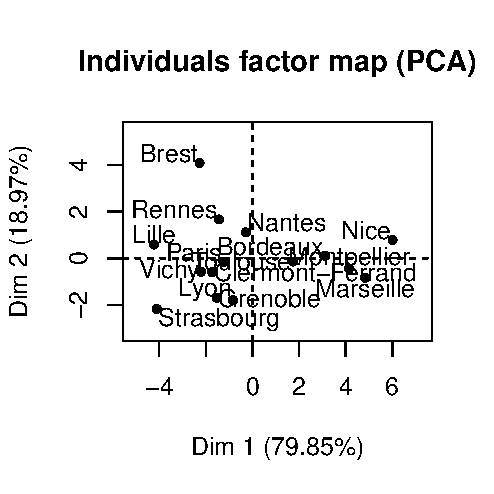
\includegraphics[width=\textwidth]{graphiques/beamer-unnamed-chunk-6-1} 

}



\end{knitrout}
\end{frame}



\begin{frame}[containsverbatim]
  \frametitle{Graphique des  individus sur les deux premiers axes}

\begin{knitrout}\footnotesize
\definecolor{shadecolor}{rgb}{0.969, 0.969, 0.969}\color{fgcolor}\begin{kframe}
\begin{alltt}
\hlkwd{cor}\hlstd{(pca}\hlopt{$}\hlstd{ind}\hlopt{$}\hlstd{coord[,}\hlnum{1}\hlopt{:}\hlnum{2}\hlstd{],temp[,}\hlkwd{c}\hlstd{(}\hlstr{"lati"}\hlstd{,}\hlstr{"long"}\hlstd{)])}
\end{alltt}
\begin{verbatim}
##             lati       long
## Dim.1 -0.8389348  0.1714839
## Dim.2  0.3064996 -0.7922192
\end{verbatim}
\end{kframe}
\end{knitrout}
\end{frame}

\begin{frame}[containsverbatim]
  \frametitle{Graphique des  individus sur les deux premiers axes}

  A partir des donn�es et des r�sultats de l'ACP, nous avons pu retrouver
  la lattitude et la longitude approximative.
  

\end{frame}

\end{document}

